% kapitel2.tex
\chapter{Fundamentals and Background}
\label{chapter:fundamentals}

As stated in the \href{chapter:introduction}{introduction}, most routing algorithms focus on shortest paths between two or more points.
Many of those have been reviewed in several different surveys (see for example \cite{madkour_survey_2017, wayahdi_greedy_2021}).
Additionally, there have been many more heuristic approaches, like local search variants \cite{braysy_vehicle_2005, irnich_sequential_2006, ropke_heuristic_2005} or different neighborhood based ideas \cite{braysy_vehicle_2005, irnich_sequential_2006, ropke_heuristic_2005} that offer faster results in exchange for not necessarily finding the one best solution, but only close approximations.
Much research has been done and is still ongoing for these kinds of problems, stemming from the fact that many graph routing problems (for example the traveling salesman problem (TSP) \cite{gendreau_handbook_2010}, the vehicle routing problem (VRP)  \cite{braysy_vehicle_2005, irnich_sequential_2006} or the arc orienteering Problem (AOP) \cite{agarwal_correlated_2023, buchin_tour4me_2022}) are NP-hard \cite{reinelt_traveling_2003}.
 
Furthermore, finding a shortest path is important in various parts of daily life.
Whether the problem is discovering the best (shortest, quickest, most convenient) way to get to work or to a supermarket by car or bike, a good way to minimize travel time by bus or any other trip from one place to another.
The examples for shortest path problems are numerous.
Additionally, shortest paths are not limited to real-world networks but can also prove useful for social networks or any form of digital network \cite{potamias_fast_2009}.
Here, different algorithms can help calculating friend networks or support the routing of data through virtual networks. 

\section{Arc Orienteering Problem}
\label{sec:aop}

The arc orienteering problem (AOP) is a variant of the orienteering problem (OP) and forms the central concept for roundtrip generation.
Souffiau et al.\ \cite{souffriau_planning_2011} describe the problem and underlying ideas as well as basic definitions of the AOP in detail.
While many other variants of the OP mainly use the nodes of a graph to determine the benefit, the AOP focuses specifically on arcs - the edges - of the graph.
Here, the underlying question is to generate a path that maximizes the profit of the contained edges while staying within the bounds of a maximum length ($C_{max}$). 
Each edge has a cost $c_{ij}$ and a profit $p_{ij}$, which contribute to the overall length and overall profit of the generated path.
The maximum length has to be defined by the user.
Furthermore, a start- and endpoint have to be determined.
For roundtrips, these two points are defined by the same vertex, so only the starting point $s$ needs to be selected.

In a graph $G=(V,E)$, vertex positions are denoted by $v_{ij}$.
Whether an edge is part of a path or not is given by $\chi_{ij}$
Based on Souffiau et al., the objective is to maximize 

\begin{equation}
	\label{eq:aopMaximize}
	\sum_{i=1}^{n} \sum_{j=1}^{n} c_{ij} \chi_{ij}
\end{equation}

while adhering to the following constraints:


\begin{equation}
	\label{eq:aopConstraints1}
	\sum_{j=2}^{n} \chi_{1j} = \sum_{i=1}^{n-1} \chi_{in} = 1
\end{equation}
\begin{equation}
	\label{eq:aopConstraints2}
	\sum_{i=1}^{n} \chi_{ik} =  \sum_{j=1}^{n} \chi_{kj} \leq 1 \;\;\; \forall k = 2,...,n-1
\end{equation}
\begin{equation}
	\label{eq:aopConstraints3}
	\sum_{i=1}^{n}  \sum_{j=1}^{n} \chi_{ij} \leq C_{max}
\end{equation}
\begin{equation}
	\label{eq:aopConstraints4}
	2 \leq v_i \leq n \;\;\; \forall i = 2,...,n
\end{equation}
\begin{equation}
	\label{eq:aopConstraints5}
	v_i - v_j + 1 \leq (n-1)(1-\chi_{ij}) \;\;\; \forall i,j = 2,...,n; \;\;\; i \neq j
\end{equation}
\begin{equation}
	\label{eq:aopConstraints6}
	\chi_{ij} \in \{0,1\} \;\;\; \forall i,j=1,...,n
\end{equation}


The first constraint (\ref{eq:aopConstraints1}) ensures that both the starting point as well as the end point are part of the resulting path.
For roundtrips, this constraint can be simplified to only use the first or the last point.
The second constraint (\ref{eq:aopConstraints2}) establishes that the resulting tour is connected.
Furthermore, all the contained vertices and edges have to be visited.
The third constraint (\ref{eq:aopConstraints3}) guarantees that the resulting path will be at most of length $C_{max}$.
While constraints four and five (\ref{eq:aopConstraints4}, \ref{eq:aopConstraints5}) ensure that no sub-tours are created.
The last constraint (\ref{eq:aopConstraints6}) defines the permissible values (0 and 1) $\chi$ can have.
These values indicate whether the edge is part of the solution (1) or not (0). 


Using these constraints and the base formula (\ref{eq:aopMaximize}) to be maximized, the arc orienteering problem can be solved by various different algorithms.


\section{Shortest Path algorithms}
\label{sec:shortestPath}

Despite not being directly usable for solving roundtrip problems, shortest paths still form an important background for the rest of the thesis. 
Shortest path algorithms have been studied extensively for many years.
In 1994, Deo and Pang \cite{deo_shortest-path_1984} created an overview tree for different types of shortest path sub-classes to give a better overview how to systematically classify a certain question into one of these categories.
The tree is visualized in figure \ref{fig:shortestPathTaxonomy}.
This visualization gives a first idea of how complex the shortest path problem can be and how many different types of questions arise in different networks and with different goals.


\begin{figure}[ht]
	\centering
	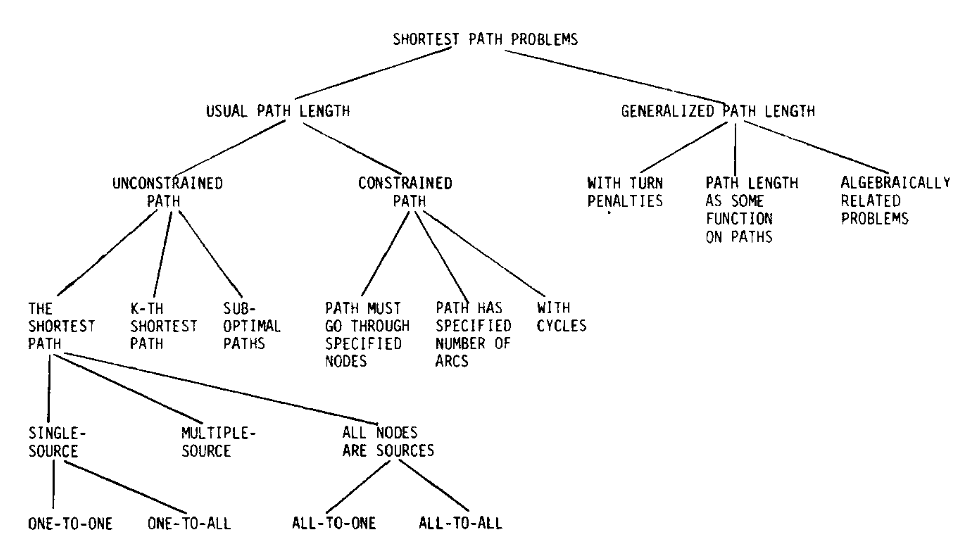
\includegraphics[width=\linewidth]{bilder/shortest path variants tree (Shortest-path algorithms Taxonomy and annotation).png}
	\caption{This image shows a conceptual tree of different variations of shortest path algorithms, taken from \cite{deo_shortest-path_1984}}
	\label{fig:shortestPathTaxonomy}	
\end{figure}

Since the shortest path problem has been well-studied and still continues to advance in terms of the quality of the returned paths as well as in optimizing the running time of algorithms, the number of approaches to solve this problem is enormous.
The above tree offers a systematic approach to classify problems and most fall into one of two categories: they are either single-source shortest paths (SSSP, on the leftmost branch the two bottom left items) or all-pairs shortest paths(APSP, on the leftmost branch the two bottom right items).


The first  - SSSP - only uses one single starting point and tries to find the one shortest path between this point and one or all other vertices.
These kinds of problems have common use cases in many daily routing problems. 
One to one paths are already described in this chapter's introduction - finding shortest paths to a specified destination \cite{sanders_shortest_2019}.
One to all paths can be useful for cases like fire departments or the police that might need a map of quickest routes for every place in their jurisdiction \cite{sanders_shortest_2019}.

The second aims to find shortest paths between all vertices of a graph - starting from a specified vertex or from every vertex to every other, which can be necessary for transportation networks and similar use cases. 
All to one path calculations can be useful in scenarios where an accident happens and out of all available emergency vehicles, the ones with the shortest paths have to be determined \cite{khamayseh_efficient_2015}.
For all to all paths, many traffic-load calculation problems come to mind. 
For example cases where trains have to be distributed along the rail network \cite{curtis_rewire_2012}.


Aside from these two categories, many more can be found to describe and sort types of approaches. 


Which of these shortest path algorithms performs best is typically dependent on the type of graph the implementation is being used on, the graph's structure and the specific problem to be solved. 
A graph can be categorized as planar or not, directed or undirected, weighted or not, and carry only non-negative weights or allow negative ones as well, they can contain cycles or be acyclic and many more. 
These different types determine which algorithms can be used as well as which will return better results.
Some algorithms like Dijkstra can - without modifications - only be used on a specific type of graph. 
In this case, the graph needs to have only non negative edges.
Others are modified versions, created specifically to fix problems like graphs with negative edges. 


\section{Heuristic Approaches}
\label{sec:metaHeuristics}

Additionally to exact approaches, heuristics can be used to improve the runtime of an algorithm.
A heuristic is a technique that is based on experience or statistical insights \cite{gendreau_handbook_2010}.
The downside of using such an approach is, that there will no longer be a guarantee that the result is the global optimum, as heuristics specifically only find partial or approximate solutions to a given problem. 
In many cases where exact algorithms would take too much time or space to find the actual optimal solution, heuristics can be used to find the best possible solution within the given bounds.

For these heuristics, several different ideas have been formed. 
These can then be categorized into construction heuristics, improvement heuristics and meta-heuristics \cite{laporte_5_2002,ropke_heuristic_2005}.
However, differentiating between these different types is not always trivial and oftentimes, the line is blurred.

Construction heuristics build their solution from a starting point until a certain boundary is reached. 
They typically don't have a separate improvement phase.
Improvement heuristics try to improve an already existing solution.
They perform improvement steps several times until a specified boundary is reached.
These boundaries can be e.g. a time limit or reaching the threshold for a good enough approximation.
(Iterative) Local Search and Neighborhoods are examples of improvement heuristics that can be used to reach a more optimized solution.

Meta-heuristics are a form of heuristic approaches.
As such, they also try to find an approximate solution to a problem that is as optimal as possible.
The distinction between classical heuristics and meta-heuristics is, that the latter are combined with additional strategies.
These are used to enable the meta-heuristics to not produce only solution that are locally optimal, but to broaden the search space they can use for finding optima.

Classical heuristics oftentimes carry the inherent risk of only finding a local optimum that can be far from the actual global one.
To reduce this risk, higher level approaches are necessary.
These can include using several neighborhood structures to broaden the search space or entirely new concepts like the Ant Colony approach or Genetic Algorithms. 

The meta-heuristic ideas that will be used in this thesis will be explained in the following subsections.



\subsection{Ant Colony}
\label{subsec:antColonyBackground}

Ant Colony is a meta-heuristic approach that is based on biological ants, ant colonies and how they search food.
Real ants start off by walking around on random paths starting from their nest. 
When they discover a food source, they pick up the food and walk back to their nest.
On this way, they distribute a substance called pheromones.
These can then be detected by other ants and indicate to them, that a path leads to a potentially good food source. 
Other ants then are more likely to follow a path with more pheromone placed on the respective edges and will in turn lay down their pheromone as well, leading to an accumulation of the pheromones on good paths.
Over time, the pheromones dissipate and when they aren't renewed, will evaporate completely, decreasing the attractiveness of the corresponding path \cite{gendreau_handbook_2010, dorigo_ant_1996}. 

Furthermore, pheromone distribution also inherently leads to using shorter paths. 
When several ants have to choose between paths, they will first select at random.
However, as soon as one ant discovers the food, turns around and distributes pheromone on the way back, this process automatically increases the likelihood of the respective path being taken by other ants.
Here, the shorter paths will be first to receive more pheromones as the ants returning will be quicker.
Due to the faster accumulation, more ants will choose this shorter path and thus place even more pheromone on it, leading to a self-reinforcing loop that converges when all ants choose the best path only.
Then, all worse paths will loose all their pheromone over time and leave the best result as the only remaining path \cite{gendreau_handbook_2010, dorigo_ant_1996}.

To illustrate pheromone distribution, an example illustrates in figure \ref{fig:antSystemExampleIllustration} how real ants find food and establish the best path towards the source. 
In part \textbf{a} on the left side, there are many ants that run between two points A and E. 
These could be the nest and an interesting food source.
In part \textbf{b} in the middle, an obstacle has been added.
This construction now leaves the ants with a choice, which path to follow. 
In the beginning, the likelihood of picking either path will be around 50\%.
While taking the path, the ants distribute pheromones on it. 
On the shorter route, the ants will end up reaching the food source earlier, thus returning quicker than the ones who took the long path and distribute more pheromone on the shorter path.
For the first few ants, there will be almost no change in the attractiveness of either path.
However, the more ants take the short tour and return quicker, the more pheromone will accumulate on that path.
This new pheromone placement and distribution leads to a shift in the attractiveness, making the shorter path more likely to be chosen by later ants.
These ants will in turn again increase the amount of pheromones placed, making the path even more attractive.
Thus, the ants create a self-reinforcing loop of positive feedback through their pheromones which eventually leads to a state where all ants always choose the shorter option.


\begin{figure}[H]
	\begin{centering}
		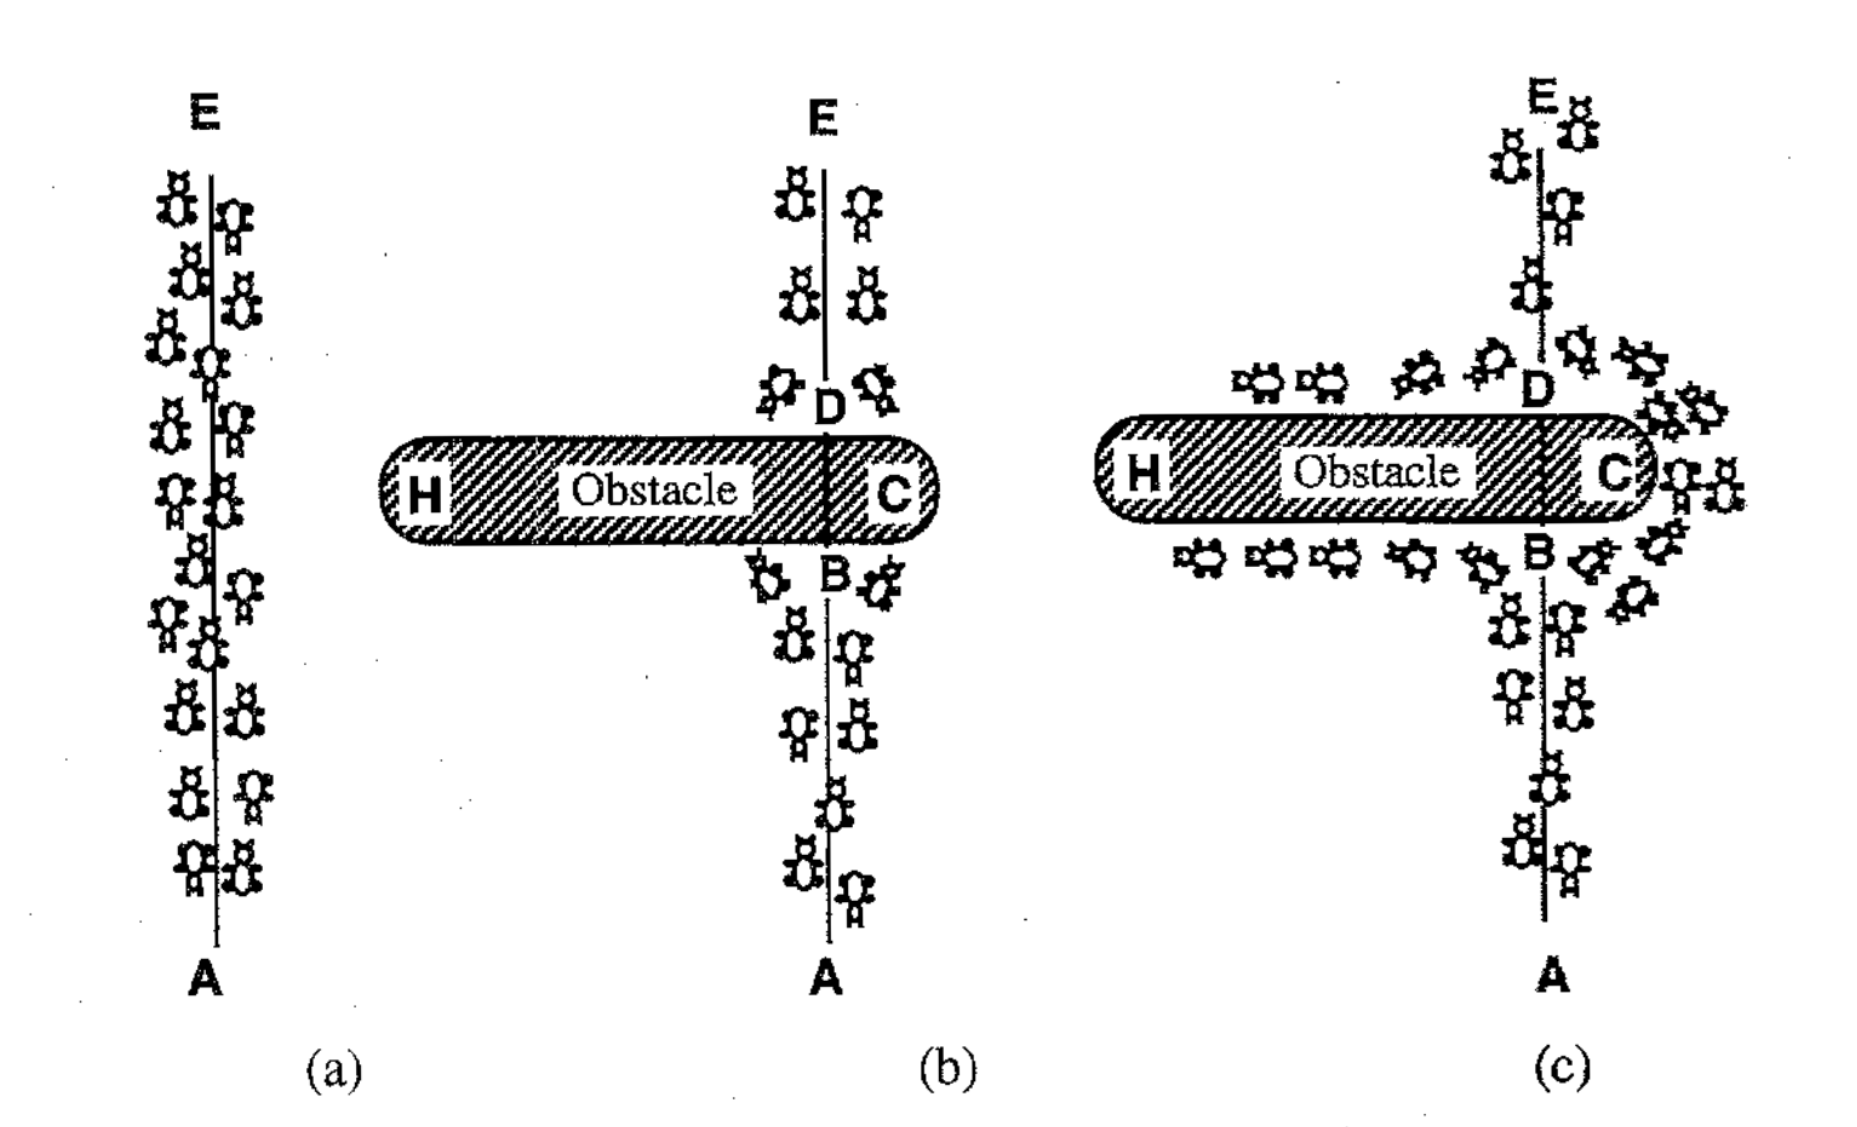
\includegraphics[width=0.8\textwidth]{bilder/antSystemExampleIllustration.png}
		\caption{This figure shows an example of pheromone distribution with real ants. Taken from \textit{Ant System: An Optimization by a Colony of Cooperating Ants}\cite{dorigo_ant_1996}}
		\label{fig:antSystemExampleIllustration}
	\end{centering}
\end{figure}


This behavior can be replicated in virtual graphs for various routing problems.
Ant system has been first introduced in 1990 by Dorigo et al\cite{dorigo_ant_1996}.
In the paper, the authors describe how to use ants for solving the traveling salesman problem (TSP).
This problem is different from the question of finding a roundtrip with a certain length (plus additional user preferences).
However, in the paper, they stress the adaptability of ant system approaches, showing both versatility and robustness on different example problems\cite{dorigo_ant_1996}.


\subsubsection{Calculations}
\label{subsubsec:antCalculations}

To transform the analogy of real ants into an algorithm, some formulas and calculations are needed.
Ants are very simple agents. 
They can only do two things:
Pick the next node to move to and place pheromone on a path.
They communicate with other ant agents through the pheromone trails, making this process a decentralized way of communication without the need for a central agent.
For the algorithm, a set amount of $m$ ants moves through the graph, tries to find a good tour and places pheromones on edges.
Every ant has a defined amount of pheromone to place. 
How much of the pheromone will be laid on a path can be calculated in several different ways. 
Dorigo et al propose the following three ideas\cite{dorigo_ant_1996}:

\begin{equation}\label{eq:antCycle}
	\Delta\tau_{ij}^k = \begin{cases}
			\frac{Q}{L_k} &\text{if (i,j) $\in$ tour described by $tabu_k(1)$} \\
			0 &\text{otherwise}
	\end{cases}	
\end{equation}


\begin{equation}\label{eq:antDensity}
	\Delta\tau_{ij}^k = \begin{cases}
	Q &\text{if the kth ant goes from i to j between time} \\
	&\text{t to t+1} \\
	0 &\text{otherwise}
\end{cases}	
\end{equation}


\begin{equation}\label{eq:antQuantity}
	\Delta\tau_{ij}^k = \begin{cases}
	\frac{Q}{d_{ij}} &\text{if the kth ant goes from i to j between time} \\
		&\text{to t+1} \\\
	0 &\text{otherwise}
\end{cases}	
\end{equation}

Here, equation \ref{eq:antCycle} is the default the authors used for solving the TSP.
The constant Q has to be picked according to the problem in question.
Variable $L_k$ describes the length of the whole tour.
This property makes sense for the TSP setting, but is relatively useless for the case of tours with a fixed length, as it will be the same value for every ant and every run made.
In this case, where the user defines the length of the tour, $L_k$ will only scale the values picked for Q\cite{dorigo_ant_1996}.

Equation \ref{eq:antDensity} only uses the constant Q to describe pheromone placement. 
Here, neither the full tour length nor individual edge costs are taken into account. 
Pheromone is placed evenly on all edges.
This way of placing pheromones equates to a not-scaled version of equation \ref{eq:antCycle} with the given use-case of a set length for the tour\cite{dorigo_ant_1996}.

The last equation \ref{eq:antQuantity} divides the constant by the length - or the cost - of each edge when it is used. 
This division reduces the amount of pheromone placed on longer edges proportionally to shorter edges. 
While this equation is not influenced directly by the fixed length, this property can still cause the equation to be less useful for tours with a specified length than for TSP.
Since tours that are meant to cover a fixed distance are different from the TSP, where a shortest path that visits all selected cities is to be found, the last equation seems like the least promising candidate for useful pheromone distribution\cite{dorigo_ant_1996}.

The pheromone calculation and placement can be defined with different formulas depending on the problem and what should be optimized. 
Which option turns out to be the best fitting one will be described in the evaluation chapter \ref{chapter:evaluation}.


Using a suitable formula to calculate the pheromone distribution, this value can then be used to calculate the overall distributed pheromone for each edge $(i,j)$ that was placed by all ants during one iteration.
This value is described by $\Delta\tau_{ij}$ as follows\cite{dorigo_ant_1996}:

\begin{equation}\label{eq:deltaTau}
	\Delta\tau_{ij} = \sum_{k=1}^{m} \Delta\tau_{ij}^k 
\end{equation}

This overall value can then be used to calculate the so called al.\ intensity\grqq{} of the placed pheromone trail.
Since pheromones evaporate over time, this property has to be modeled as well, using a new parameter $\rho$, which describes how much of the pheromone stays on the trail between two time steps.
Thus, the overall pheromone intensity can be described by


\begin{equation}\label{eq:trailIntensity}
	\tau_{ij}(t+n) = \rho \cdot \tau_{ij}(t)+\Delta\tau_{ij}^k 
\end{equation}

where $\tau_{ij}(t)$ is the previous pheromone intensity and t+n describes the next time step after one full tour was created in n steps\cite{dorigo_ant_1996}.

Using these calculations, the pheromone intensity on all paths can be represented. 
What's left is determining the probability with which ants will choose a certain edge over the other options.
For this calculation, two more properties are needed: the visibility of an edge and a tabu-list (or rather a list of allowed nodes).
The tabu-list contains all nodes that have been visited before.
Since roundtrips should - per default - be round rather than the same path run in two directions, this property is needed to ensure no city is visited more than once.
In chapter \ref{chapter:evaluation}, different configurations are tested to represent different shapes and allow for more options users can define. 
Thus, for other shapes, this list is not needed.
The visibility $\nu_{ij}^k$ is calculated using the length of the edge $d_{ij}$ as follows:

\begin{equation}\label{eq:visibility}
	\nu_{ij}^k = \frac{1}{d_{ij}}
\end{equation}

And the transition probability is given by

\begin{equation}\label{eq:transitionProbability}
	p_{ij}^k = \begin{cases}
		\frac{[\tau_{ij}(t)]^{\alpha} \cdot [\nu_{ij}]^{\beta}}{\sum_{k \in allowed_k} [\tau_{ij}(t)]^{\alpha} \cdot [\nu_{ij}]^{\beta}} &\text{if $j \in allowed_k$ }\\
		0 &\text{otherwise}
	\end{cases}
\end{equation}

using all previously defined values to calculate visibility $\nu_{ij}^k$, trail intensity $\tau_{ij}$, pheromone distribution $\Delta\tau_{ij}$ and $\Delta\tau_{ij}^k$.
Here, $\alpha$ and $\beta$ are parameters that influence the weight of visibility and trail intensity.
Higher values of $\alpha$ increase the significance of the pheromones on the trail (setting $\alpha$ to 0 would lead to completely ignoring the pheromone placed) and higher values of $\beta$ increase the importance of the visibility of an edge (making longer edges less attractive as a result)\cite{dorigo_ant_1996}.
These parameters will be experimented with and their influence will be evaluated in chapter \ref{chapter:evaluation}.

In their paper, Dorigo et al suggest middling values for $\alpha$ and $\beta$ in a range of $[0.5,5]$.
They furthermore stated that the best tour was achieved using $\rho = 0.5$ and $Q=100$.
Overall, the results of experimenting with different parameter configurations showed that for very high or very low values of $\alpha$, no good results could be generated \cite{dorigo_ant_1996}.



\# TODO add formulas and description how they help constructing paths
\# TODO add how to use for my work


\subsubsection{Pseudocode}
\label{subsubsec:antPseudocode}

\subsection{Simulated Annealing}
\label{subsec:simulatedAnnealingBackground}

Simulated Annealing (SA) builds upon a statistical physics concept of annealing.
The physical process of annealing describes a thermal procedure to improve solids.
Improving in this case means \enquote{obtaining low energy states of a solid in a heat bath} \cite{aarts_simulated_2005}.
Low energy is needed to achieve the stable solid state of a crystal \cite{delahaye_simulated_2019}, see figure \ref{fig:annealingIllustration} for a visualization of the different states.

The physical process is split into two general steps:
\begin{itemize}
	\item melting the solid through heating
	\item cooling the material to a specified temperature
\end{itemize}
The basic concept is, that given a sufficiently high starting temperature to which the material is heated and a long enough cooling time, the material can reach a stable solid state. 

\begin{figure}[h]
	\centering
	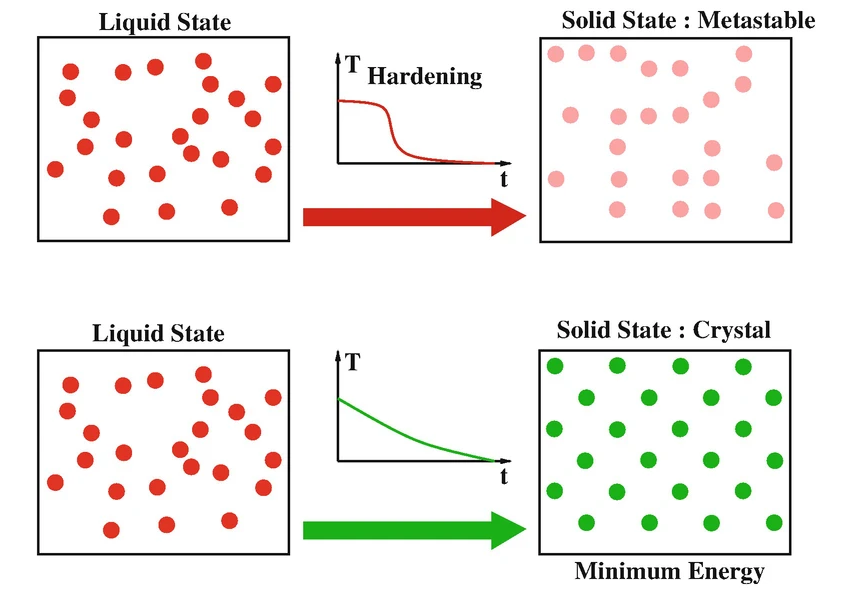
\includegraphics[width=0.9\textwidth]{bilder/AnnealingIllustration.png}
	\caption{The illustration shows two different cooling procedures for a material. The upper one depicts the effects of sudden cooling, resulting in a meta-stable state, while the lower one portrays a slower cooling schedule which results in a stable solid state \cite{delahaye_simulated_2019}.}
	\label{fig:annealingIllustration}
\end{figure}


The above figure shows the effects of different cooling schedules on a material and the type of solid state this material will obtain as a result.
In the upper part, the top left image shows a liquid state, in which molecules are free and can move around.
Cooling down too quickly hinders the atoms to move into proper positions, resulting in an unordered, non-symmetrical state, which is meta-stable (top right).
In contrast, the lower part depicts a slower cooling process, where the atoms are given enough time to move into symmetrical form (bottom right).
This state is equivalent with a minimum energy state, resulting in a stable crystal structure and a highly durable solid material. 

Based on this analogy, simulated annealing was developed as a concept to solve NP-hard computational problems by improving local search variants \cite{aarts_simulated_2005, eglese_simulated_1990}.
Local search approaches a very good at finding locally optimal solutions, but can easily fail to find a global optimum.
Simulated annealing addresses this problem with the underlying idea based on the two steps of heating and slow cooling.
What makes SA different from a basic local search is, that it allows -- with a certain probability (temperature) -- for worse solutions to be accepted.

First, some basic solution for the problem is needed.
For the use case of this thesis, a basic solution will be a roundtrip.
Furthermore, a function which determines the quality of the solution is needed, so that comparing different solutions to each other is possible. 
Starting from the initial roundtrip, neighboring solutions need to be generated and their quality will be assessed using the quality function.
Any neighboring roundtrip which yields a better result will be accepted as the new solution that has to be improved.
Worse roundtrips can also be accepted based on a cooling schedule.

The schedule contains an initial temperature and a function to calculate the cooling of this value, lowering it over time.
In the beginning, the solution is likely to be further away from a global optimum.
Thus, a higher temperature allows for an increased likelihood to accept solutions with a lower quality, which in turn allows to escape local optima.
The longer SA runs, the lower the temperature gets, lowering the likelihood of accepting worse solutions while nearing the global optimum. 
To do this, several nested runs are needed.
In an outer loop, the temperature changes and gets updated with lower values.
In an inner loop, several possible neighborhoods are tested for one temperature state. 
Solutions that are better than the previous one are always chosen.
Solutions that are worse than the previous one are chosen based on the temperature.


For SA to yield a good result, several parameters need to be set. 
First, a starting roundtrip, which builds the base, has to be calculated.
Then, initial temperature as well as the cooling formula have to be determined.
Furthermore, a neighboring roundtrip has to be found, as well as a formula for calculating the quality of all found solutions.
Additionally, the number of runs has to be decided, while keeping both the runtime as well as the quality of the resulting tour in mind.

For some of the parameters -- like the initial temperature and the cooling formula --, thorough testing of different configurations is needed.
For others, only a limited set of options is interesting.
Determining a neighboring roundtrip as well as an initial solution are the two parameters that have a narrow array of possibilities to calculate them.

For an initial solution, the implemented algorithms -- AntColony, Greedy and MinCost (see \ref{subsec:Tour4Me}) -- can calculate a base roundtrip.
Which of these is to be preferred is dependent on the preferences about the resulting shape. 
Greedy and AntColony prioritize edge quality while MinCost mostly optimizes for a rounder shape.

To determine a neighboring solution, there are a few options that can yield good results.
One approach is to pick two random vertices and switch their position in different ways within the roundtrip path \cite{zhan_list-based_2016}. 
Another is to create waypoints, similarly to how it is done in the MinCost algorithm, but without the length restrictions.
The generated initial solution can then be used to generate a set of waypoints. 
Based on this node set, neighboring roundtrips are ones where the tour is modified by removing, adding or moving one of the waypoints.

To remove a waypoint, the node and the paths that connect this vertex with the neighboring two waypoints need to be deleted. 
Then, the two ends are connected by a shortest path or a MinCost approach.
For adding a waypoint, first, a suitable node needs to be determined. 
This choice can be done either randomly or based on a probability distribution that gives higher probabilities to nodes closer to the path and lowers in value the further away a node is.
After a suitable node was picked, the closest waypoint and the best neighbor needs to be found.
This selection is done by calculating the shortest paths from the new waypoint to all existing ones.
Then, the connection between the two picked nodes has to be removed and a the new waypoint needs to be joined up with the two nodes that now frame the gap. 
Moving is the combination of removal and adding.
For this operation, the new node has to be found first and the closest waypoint will be the one to remove.




\subsubsection{Calculations}
\label{subsubsec:SACalculations}

For SA, a few parameters have to be calculated.
The temperature schedule can be calculated using an exponential function to decrease the value for each iteration, where f(j) is the quality of the neighboring solution, f(i) the quality of the current solution and T the temperature: 

\begin{equation}\label{eq:temperatureSchedule}
	T = e^{\frac{f(j)-f(i)}{T}}	
\end{equation}

The quality of the solution is calculated based on the covered area A and the respective importance (areaImportance), the edge profit (P) and the respective importance (edgeImportance) and all other valuable properties (others) and scaled by the target length of the tour (L). 

\begin{equation}\label{eq:qualitySA}
	f(i) = \frac{areaImportance * A(i)}{\pi * L(i)^2} + \frac{edgeImportance * P(i)}{L(i)} + others(i)
\end{equation}


\subsubsection{Pseudocode}
\label{subsubsec:SAPseudocode}



\begin{algorithm}
	\caption{High level Simulated Annealing}
	\label{alg:SApseudocode}
	\begin{algorithmic}[1]
		\STATE Select init roundtrip (i)
		\STATE Select init temperature (t)
		\FOR{$i=0$ to numberRepitions}
			\FOR{$i=0$ to numberRuns per temperature}
				\STATE Generate neighborhood roundtrip (j)
				\STATE Calculate difference in quality d = f(j)-f(i)
					\IF {d $\geq$ 0}
						\STATE use neighboring solution as current best i $\gets$ j
					\ELSE 
						\STATE random $\gets$ generate random(0,1)
						\IF {random < exp(d/t)} 
							\STATE use neighboring solution as current best i $\gets$ j
						\ENDIF
					\ENDIF
			 \ENDFOR
			 \STATE update temperature t $\gets$ T(t)
		 \ENDFOR
	\end{algorithmic}
\end{algorithm}










\subsection{Genetic Algorithms}
\label{subsec:geneticAlgorithmsBackground}



